\documentclass[10pt]{academydoc}
\pagestyle{plain}

% Set Document Details
\doctype{tb} % spec, proc, tb (Specification, Procedure, Technical Bulletin)
\docname{Academy Color Encoding System Version 1.0\\*User Experience Guidelines}
\altdocname{ACES Version 1.0 User Experience Guidelines}
% Sets the document name used in header - usually an abbreviated document title
\docnumber{TB-2014-002}
\committeename{Academy Color Encoding System (ACES) Project Committee}
\versionnumber{1.0.2}
\docdate{September 3, 2015}
\summary{
The Academy Color Encoding System (ACES) is the industry standard for managing color throughout the life-cycle of a motion picture or television production (from creation, thru editorial, grading, audience presentation, and archiving).

Early adopters of technology products tend to be quite technology-savvy. One of the main goals of the release of ACES 1.0 is to broaden the user base beyond the very technically-oriented early adopters. In order to make it more accessible to a wider audience of users, it is necessary to make the ACES User Experience (ACES UX) simpler and more consistent across products.

This document provides guidelines for those building products that implement ACES and to others looking for guidance on how best to present ACES terminology and concepts to end-users.

Those implementing ACES in products should also refer to the Logo Program Requirements and Usage document.
}

% Document Starts Here
\begin{document}

\maketitle

% This file contains the content for the Notices
\prelimsectionformat	% Change formatting to that of "Notices" section
\chapter{\uppercase{Notices}}
%% Modify below this line %%

\copyright\the\year{} Academy of Motion Picture Arts and Sciences (A.M.P.A.S.). All rights reserved. This document is provided to individuals and organizations for their own internal use, and may be copied or reproduced in its entirety for such use. This document may not be published, distributed, publicly displayed, or transmitted, in whole or in part, without the express written permission of the Academy.

The accuracy, completeness, adequacy, availability or currency of this document is not warranted or guaranteed. Use of information in this document is at your own risk. The Academy expressly disclaims all warranties, including the warranties of merchantability, fitness for a particular purpose and non-infringement.

Copies of this document may be obtained by contacting the Academy at councilinfo@oscars.org.

``Oscars,'' ``Academy Awards,'' and the Oscar statuette are registered trademarks, and the Oscar statuette a copyrighted property, of the Academy of Motion Picture Arts and Sciences.

% This paragraph is optional.  Comment out if you wish to remove it.
This document is distributed to interested parties for review and comment. A.M.P.A.S. reserves the right to change this document without notice, and readers are advised to check with the Council for the latest version of this document.

% This paragraph is optional.  Comment out if you wish to remove it.
The technology described in this document may be the subject of intellectual property rights (including patent, copyright, trademark or similar such rights) of A.M.P.A.S. or others. A.M.P.A.S. declares that it will not enforce any applicable intellectual property rights owned or controlled by it (other than A.M.P.A.S. trademarks) against any person or entity using the intellectual property to comply with this document.

% This paragraph is optional.  Comment out if you wish to remove it.
Attention is drawn to the possibility that some elements of the technology described in this document, or certain applications of the technology may be the subject of intellectual property rights other than those identified above. A.M.P.A.S. shall not be held responsible for identifying any or all such rights. Recipients of this document are invited to submit notification to A.M.P.A.S. of any such intellectual property of which they are aware.

\vspace{10pt}
These notices must be retained in any copies of any part of this document. \newpage
% This file contains the content for the Revision History and 
\prelimsectionformat	% Change formatting to that of "Notices" section
\chapter{Revision History}
%% Modify below this line %%

\begin{tabularx}{\linewidth}{|l|l|X|}
    \hline
    Version & Date & Description \\ \hline
    1.0     & 05/10/2013 & Initial Version      \\ \hline
    1.1     & 08/02/2013 & Modify ACESproxy to handle negative ACES values \\ \hline
    2.0     & 12/19/2014 & Modify ACESproxy primaries, constrain to legal range \\ \hline
    2.0.1   & 04/24/2015 & Formatting and typo fixes \\ \hline
            &      &             \\ \hline
\end{tabularx}

\vspace{0.25in} % <-- DO NOT REMOVE
\chapter{Related Academy Documents} % <-- DO NOT REMOVE
\begin{tabularx}{\linewidth}{|l|X|}
    \hline
    Document Name & Description \\ \hline
    S-2008-001  & Academy Color Encoding Specification (ACES) \\ \hline
    S-2014-003  & ACEScc -- A Logarithmic Encoding of ACES Data for use within Color Grading Systems \\ \hline
    S-2014-004  & ACEScg -- A Working Space for CGI Render and Compositing \\ \hline
    & \\ \hline
    & \\ \hline
\end{tabularx} \newpage

\tableofcontents \newpage

% This file contains the content for the Introduction
\unnumberedformat	    % Change formatting to that of "Introduction" section
\chapter{Introduction} 	% Do not modify section title
%% Modify below this line %%

A goal of ACES 1.0 is to enable widespread adoption by encouraging consistent implementations in production and post-production tools throughout the complete film and television product ecosystem spanning capture to archiving. This is a very diverse set of tools, each used by professionals with different sets of skills. Furthermore, each manufacturer has established their own set of conventions for how to structure their user experience to best serve their market. Clearly, it is neither feasible nor appropriate for these guidelines to specify in minute detail every aspect of a user interface (e.g. ``all products must use a set of vertical drop-down menus labeled in 10-point Helvetica'').

That said, the feedback from users on the first wave of products implementing the pre-release versions of ACES has been clear in the need for guidelines. One common comment is that the implementations are so different, figuring out how to configure ACES in one product is of little help when configuring the next. For example, naming conventions are different for no apparent reason.

Another common concern is that the system is too reliant on acronyms and uses unfamiliar concepts (e.g., what is a ``reference rendering transform''?). Although some of these acronyms have become familiar within the inner circle of ACES product partners and early adopters, it must be acknowledged that the tolerance for these terms is much lower amongst the general population of industry professionals (e.g. how would one explain what an RRT is to an editor, CG animator, or anyone else without some color science background).

As the ACES project transitions from technical development to wider industry deployment and the release of Version 1.0, it is appropriate that we take a fresh look at how to portray the system to an audience that includes end-users in addition to engineers and color scientists. Although the technical terms and acronyms will continue to be used within the engineering community, these guidelines introduce a new set of terms intended to be simpler and more familiar to a wider set of users.

\note{This document provides naming conventions in English. However, it is recognized that for many products it will be necessary to translate these names into other languages to localize for various global markets.} \newpage

% This section contains the content for the References
\numberedformat
\chapter{References}
The following standards, specifications, articles, presentations, and texts are referenced in this text:
%% Modify below this line %%

Academy S-2013-001, ACESproxy -- An Integer Log Encoding of ACES Data

SMPTE ST 2065-1:2012, Academy Color Encoding Specification (ACES)

SMPTE RP 177:1993, Derivation of Basic Television Color Equations

% This file contains the content for a main section
\numberedformat
%% Modify below this line %%
\chapter{Top-level schematic for the ACES user experience}

\autoref{fig:schematic} is the overview diagram for the ACES 1.0 user experience. This is not intended to replace the earlier conceptual block diagrams. However, it must be realized that those diagrams were intended primarily for an audience of color scientists and post-production engineers rather than the much wider audience of end-users being targeted for the 1.0 release.

Notice that acronyms have been eliminated. The names have been made shorter and more intuitive (definitions are provided in \autoref{sec:terminology}).

Please note that the Output Transform is the combination of the RRT with an ODT. A diagram showing the user-centric terms in relation to the engineering-centric block-diagram is provided in Appendix \ref{appendixA}, along with definitions of the engineering terms.

\begin{figure}[htbp]
\begin{center}
    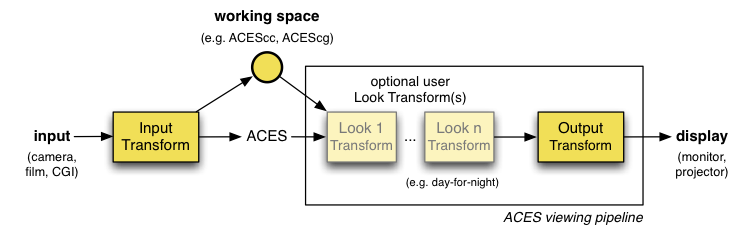
\includegraphics[width=\textwidth]{topLevelSchematic.png}
\caption{The top-level schematic for the ACES user experience}
\label{fig:schematic}
\end{center}
\end{figure}

% This file contains the content for a main section
\numberedformat
%% Modify below this line %%
\chapter{Selecting input transforms}

This section contains guidelines for selecting ACES Input Transforms. Please note that the term IDT (Input Device Transform) is also used here since it is familiar to product manufacturers, however it is important to note that this is an engineering rather than an end-user term.

\section{Challenges}
The number of manufacturers of digital cinema cameras continues to expand and each product seems to have developed its own set of UX conventions. The goal of these guidelines is not to make all camera vendors use the same set of options for their camera. Rather, it is to make the process of selecting the ACES Input Transforms for a given camera as similar as possible in the products that use those transforms.

For example, if one camera manufacturer makes IDTs that vary based on exposure index (EI), and another manufacturer makes IDTs based on whether daylight or tungsten was used (but doesn’t care about which EI was used), it is not our goal (nor would it be feasible) to get the manufacturers to all agree to use the same set of options.

Another important aspect to consider is that there is a tension between ease-of-use and completeness. On the one hand, products should make it possible for users to use any available IDT. On the other hand, given the increasing number of manufacturers, the fact that a single camera may have dozens of IDTs associated with its various parameter settings, that manufacturers regularly introduce new ``color science versions'' which may apply to new and old cameras, and the fact that the current crop of camera models gets refreshed regularly, there will soon be hundreds of IDTs available.

For users to trust in the ACES platform, they must be able to load the IDT needed for their given camera. However, for ACES to be easy to use, the user must not be overwhelmed with menus that have hundreds of different transforms. Hence product designers must somehow find a way to make their implementations both complete and yet easy to use.

Please note that as part of the ACES support effort, we plan to request that Product Partners create and publish an FAQ as a PDF that is formatted similarly (among all Product Partners of a particular category of product) to help end-users understand how a particular manufacturer is handling naming conventions and/or set-ups. These would be available on the ACES website to make it easier for users to get up and running on any particular piece of equipment.

\section{Naming of transforms}
In order to reduce ``differences for no reason,'' the transforms will contain metadata for a suggested ``user friendly'' name for use in product user interfaces (UIs). However, given the fact that ACES-compliant products will serve many different types of user and each have their own UI requirements (e.g. length of strings), it is not realistic to mandate usage of specific transform name strings. Hence, use of the proposed names is highly recommended but not mandatory.

However, one common user complaint about current pre-release ACES implementations is that it is often difficult to know if they are selecting the same transform in two different products since they are named differently.

``Academy S-2014-002, Academy Color Encoding System -- Versioning System'' is a separate document describing the process of generating versioned unique names for color transforms. Although these are human-readable, they may be too long and technical for use as the primary name in many product UIs. However this transform identifier string is the most precise way for users to confirm the ``true identity'' of a given transform (i.e. the exact CTL file that was used by the manufacturer to implement a given transform).

\section{Transform metadata}
The CTL files included in an ACES system release will contain two metadata strings that are intended for use in products:

User-friendly Transform Name -- This is the string that is recommended for use in menus, etc. in a product user interface. Some hypothetical user-friendly names are:

\begin{itemize}
	\item ACES 1.0 Input - ARRI LogC v3 (EI800)
	\item ACES 1.0 Look - ACES 1.0 to 0.7 emulation
	\item ACES 1.0 Output - P3-D60
\end{itemize}

The user-friendly transform name consists of a prefix followed by a specific name. Products may shorten the prefix if the type of transform is clear from the context.

ACES Transform Identifier (or ``Transform ID'') -- This is a versioned unique name which is fully described in Academy S-2014-002. Some hypothetical example transform identifiers are:

\begin{itemize} 
	\item IDT.ARRI.Alexa-logC-v3-EI800.a1.v1
	\item LMT.Academy.ACES\_0\_7\_1.a1.0.0
	\item ODT.Academy.P3D60\_48nits.a1.0.0	
\end{itemize}


\section{Guidelines}
\subsection{Naming of menus}
The string ``Input Transform'' (or simply ``Input'' if ``Transform'' is clear from the context) is suggested for the menu used to select IDTs. 

\subsection{Naming of transforms}
Products are free to choose the ``user friendly'' name for transforms. It is highly recommended to use (or at least base) the string on the user-friendly name metadata included in the released transforms. 

\subsection{Unique identification of transforms} \label{sec:uid1}
Products should make it possible for users to see the official transform identifier string associated with a transform. As this is a technical string, it is reasonable to put this somewhere separate from the user-friendly name (e.g., in an ``Advanced Info'' dialog box). The transform identifier may be referred to as the ``Transform ID.''

\subsection{Assigning appropriate default transforms}
In many cases, there will be information available to the product that could guide the selection of the IDT. For example, it may be an ACES clip-level metadata file, there may be other color space metadata in the image file, or the media could be in a format specific to a given camera. Where appropriate, products should attempt to simplify the user experience by selecting an appropriate Input Transform. However, since metadata unfortunately is often wrong, users should be given a way to over-ride any automatic transform selection.

\subsection{Device-specific input hierarchies}
Creators of IDTs should publish their transforms using a directory structure that provides guidance on how products should organize the presentation of these transforms to end-users. The names of the directories should be chosen carefully for suitability in products.

Products which allow users to select Input Transforms should organize the transforms using some type of hierarchical user interface metaphor to make the process of finding Input Transforms as similar as possible between products. The naming of the hierarchy should correspond to the intent of the IDT creator.

\subsection{Completeness}
Products should enable users to select any of the IDTs included in the Academy releases.

\subsection{Ease-of-use}
Products should arrange their user experience in such a way that the user is not overwhelmed by needing to select from overly long lists of transforms. One method for doing this is to have both easy and advanced modes. Another method is to present a short list of the most likely transforms but also provide a way for the user to browse to find older, less common, or more specialized transforms. (This set of suggestions is intended to be illustrative rather than exhaustive.)

\subsection{Handling other inputs}
The typical IDTs are transforms for digital cinema cameras and film scanners. However, it is important that products allow users to convert from other color spaces into ACES, even though there may not be an Academy-supplied IDT for it. For example, it is often useful to be able to convert scene-referred data encoded using the Rec. 709 primaries into ACES.

A more complicated example is the important case of importing display-referred media via an inverse Output Transform.
% This file contains the content for a main section
\numberedformat
%% Modify below this line %%
\chapter{Configuring the ACES viewing pipeline}

The most complicated aspect of the ACES user experience is configuring the settings needed for a product to convert ACES colors into device code values suitable for a given display and viewing environment.

\section{Technical background}
ACES stores images using a wide-range, linear, floating-point encoding of the original scene colorimetry. These ``scene-referred" images must be transformed for correct presentation in cinema and television. This transformation accounts not only for the difference between a linear encoding and the gamma-corrected encoding expected by display devices, but also for the difference in viewing environment between capture and display, for the limited dynamic range and gamut of practical displays, and the desire to produce a pleasing picture.

Although this transformation involves well-understood principles of color science, there are also engineering trade-offs and aesthetic considerations which means there is no single correct approach. Each product manufacturer makes the trade-offs differently which results in products producing images having their own look. Traditionally motion picture film had a specific look that was different from video cameras. In this digital era, each digital motion picture camera manufacturer has one or more looks selectable in software, while visual effects and animation companies have their own ``tone-mapping transforms" that produce customized looks serving the visual aesthetics of the production.

This diversity has created problems when interchanging digital media in scene-referred form since the recipient often does not know what viewing transform to use to correctly view the images. This has made digital workflows often more fragile than the film or tape-based workflows that they have supplanted.

One of the foundational design principles of the ACES system is that it must be possible to reasonably view ACES-encoded images on various display devices without any additional information (i.e. without knowing ``what LUT am I supposed to use?"). This greatly increases the robustness of the system, not only for exchanging files between collaborators on a project, but also for placing ACES files in the vault for future generations.

\section{The role of the Look Transform}
Prior to ACES, it was common to ``bake" a look into the output transform. This was partly due to the common limitation that many products did not allow the user to specify a separate look transform. However, ACES introduces a paradigm-shift related to look transforms.

Up to now, it has been necessary to create separate output transforms for each product being used. For example, on a large VFX movie, an engineer would need to create many flavors of LUTs in various file formats and different mathematical representations (e.g. number of grid points in the 3d-LUT, whether a pre-shaper is used or not, etc.). Furthermore, there would need to be versions for each display (e.g. transforms for both Rec. 709 and P3).

One of the benefits of having standard transforms is that product vendors can craft their implementation of the ACES transforms to perform best for how their product works (e.g. using exact math, or a specific LUT structure). Furthermore, the transforms necessary for viewing on a wide variety of displays are provided with the ACES release. Given that these will be built into the products, it is not necessary (or even desirable) to require post-production engineers to build the same type of large LUT collections.

Furthermore, ACES was designed for archiving use (similar to a negative that includes the creative color timing). Whether the Look Transform is baked in or included along with the unmodified ACES files, in either case, it is necessary for the Look Transform to exist separate and distinct from the Output Transform.

For these reasons, it is very important for products to allow users to utilize separate Look Transforms that are not combined into an Output Transform.

Ideally, products should allow the Look Transforms to be easily toggled on and off since it is often useful to see the ``neutral" or ``reference" ACES rendering on its own, without a look.

\section{Terminology} \label{sec:terminology}
ACES Output Transform -- The transform that converts ACES2065-1 colors to code values for a particular output device. This is the combination of the RRT and an ODT. (Please see Appendix \ref{appendixA} for definitions of the non-user-facing engineering terminology.)

Look Transform -- Generally, a color transformation which affects the entire image to a particular creative effect. Specifically in this context, an ACES Look Transform is the user-facing term for an LMT. The input and output color space of an ACES Look Transform is ACES2065-1. Please refer to ``Academy TB-2014-010, Design, Integration and Use of ACES Look Modification Transforms."

Viewing Pipeline -- The complete set of color transforms needed to convert color values from the product’s working space into code values to be sent to a display device. This includes the Look Transform(s) (if present), and the Output Transform. It may also include adaptor transforms needed to convert between a working space and ACES.

Working space -- The color encoding used to modify (or create) images. In other words, the color space that the algorithms (color grading, compositing, CG rendering, etc.) work in. Products typically convert each source into a common working color space, perform some operation, and then convert to another color space for display or output. In order to achieve interoperability among products, a given operation (e.g. ASC CDL) must be applied in the same working space.

\note{The terms RRT and ODT are engineering-centric terms and their use in products is deprecated.}


\section{Guidelines}
\subsection{Naming of menus}
The strings ``Look Transform" and ``Output Transform" are suggested for labeling what the user is selecting (e.g. the text next to the UI widget that contains the set of options). The word ``Transform" may be omitted if it is clear from the context.

\subsection{Naming of transforms}
Products will choose the ``user friendly" name for transforms. It is highly recommended to use (or at least base) the string on the user-friendly name metadata included in the transform files. The recommended name for the Output Transform is contained in the ODT transform file. 

\subsection{Unique identification of transforms} \label{sec:uid2}
Products should make it possible for users to see the official transform identifier string associated with a transform. As this is a technical string, it is reasonable to put this somewhere separate from the user-friendly name (e.g., in an ``Advanced Info" dialog box). The transform identifier may be referred to as the ``Transform ID."

Because the transform identifier for ODTs is incremented whenever the RRT changes, for the Output Transform it is sufficient to provide the transform identifier from the corresponding ODT.

\subsection{Completeness}
Products should enable users to select any of the Output Transforms included in the Academy releases.

\subsection{Ease-of-use}
Products should arrange their user experience in such a way that the user is not overwhelmed by needing to select from overly long lists of transforms. One method for doing this is to have both easy and advanced modes. Another method is to present a short list of the most likely transforms but also provide a way for the user to browse to find older, less common, or more specialized transforms. Another method is to filter the list of options. (This set of suggestions is intended to be illustrative rather than exhaustive.)

\subsection{Handling other outputs}
If in addition to viewing media on a display, the product also allows users to create new files, it may be necessary to allow the user to bake in an Output Transform that is different from the one they are using with their current display. For example, the user creates content on a broadcast monitor but needs to produce output for web viewing (i.e. sRGB).

Also, in some products it is useful to allow other options. For example, in some VFX use-cases it is necessary to deliver media in the same format as the originals. In this scenario it is useful to allow an inverse IDT to be applied on output. (It is hoped that over time, this use-case will no longer be necessary and files may be exchanged using the ACES2065-1 encoding and ACES container format.)

\subsection{Assigning appropriate default transforms}
In many cases, there will be information available to the product that could guide the selection of the Output Transform. For example, the user may have already indicated elsewhere in the UI or during the installation/setup of the product what display device is connected. Also, it may be possible for a product to default to the most appropriate Output Transform based on the context (e.g. the user is doing video mastering). However, users should always be provided a method to over-ride any automatic transform selection.

\subsection{Separate Look Transforms}
The Look Transform is an integral part of the ACES system and products should enable users to select one or more Look Transforms to be applied in the viewing pipeline before the Output Transform. It is important to support the case where the Look Transform is separate from the Output Transform.
% This file contains the content for a main section
\numberedformat
%% Modify below this line %%
\chapter{Versioning}

Anyone who has followed the rapid development of digital cinema technology is familiar with the fact that manufacturers regularly revise their color science as the state of their technology advances. For example, several of the leading digital camera manufacturers are already at version 3 or higher of their color science. As may be seen in the products that support their SDKs, each has their own method of indicating version choices.

Likewise, given the challenges in developing a color management framework that meets the needs of all parts of the industry, it is expected that version 1 of ACES will not be the last. By provisioning for this eventuality now, it is hoped that some amount of confusion may be lessened in the future.

Furthermore, it is anticipated that many products will want to support the pre-release ACES versions for some additional period of time to support users with projects created with the pre-release transforms.

Therefore, the ACES UX design needs to clearly identify which version of ACES is being used and the method should be as similar as possible amongst implementations.

Each of the components of ACES will be versioned and there is also a version assigned to each ACES Release (consisting of transforms, specifications, and guidelines). See ``Academy S-2014-002, Academy Color Encoding System -- Versioning System'' for further details.

The ACES components have version numbers with major, minor, and (in some cases) patch components. Product manufacturers should keep in mind that end-users will not be familiar with the detailed semantics of ACES versioning and should take care to show an appropriate level of detail. All components built for a given ACES System version must be compatible with each other. Therefore, in some contexts it may be desirable to only show the major, or major and minor, parts of the version.

\section{Guidelines}
\subsection{Display of ACES Release version}
Users should be shown the ACES Release version being used in the product. At a minimum this should also be used in the name of the ACES Output Transforms.

The suggested end-user string for the first official ACES Release is ``ACES 1.0.''

The suggested end-user strings for pre-release versions of ACES are ``ACES 0.1,'' ``ACES 0.2,'' and ``ACES 0.7.''

\subsection{Use of appropriate default versions}
For new work, the current version of ACES should be the default. It is suggested that products somehow structure the UX so that users are guided to select transforms for the current version, e.g., by filtering the transform options so that users ``see the current version first.'' 

When loading work based on earlier platform releases, the transforms for that release should continue to be used.

\subsection{Availability of earlier ACES Releases}
Products should allow users to access all of the ACES Releases. For example, even after ACES 3.0 comes out, users should still be able to use ACES 1.x and ACES 2.x transforms. This may (and, in fact, should) require more work from the user than accessing the current version.

Support for the pre-release versions of ACES is suggested but optional.

\subsection{Display of ACES Transform Identifier}
Products should provide a way for users to see the ACES Transform Identifier string associated with a transform they have selected via the UI (see \autoref{sec:uid1} and \autoref{sec:uid2}).
% This file contains the content for a main section
\numberedformat
%% Modify below this line %%
\chapter{Naming of color spaces and encodings}

The pre-release versions of ACES focused heavily on the transforms from input devices and the transforms to output devices. However, the overall user experience of ACES goes beyond these device color transforms. If the working space used in a product is not properly chosen, this can easily cause problems for users.

A full discussion of working spaces and color encodings is beyond the scope of this document and a proper introduction to those topics will be provided in a separate document. However, this section provides a concise description intended to set the necessary context for the UX requirements.

As defined above, a working color space (or working space) is the digital representation of color that a product uses to edit or create images--it is the representation manipulated by the algorithms that embody the product. In the field of color science, a color encoding specification is a method for digitally encoding color that is used to communicate a color appearance. The specification should include information such as the color primary set and the non-linearity (if any) applied prior to digital quantization. This essentially provides a mapping between the digital code value and a color stimulus. In addition, it is important that the specification also describe the intended viewing environment so that the appearance of that color stimulus may be estimated.

The SMPTE 2065-1:2012 color encoding specification is not always the most appropriate choice for a working space. Indeed, the use of the ACES color transforms does not require that the 2065-1 space be used as the working space.

In some pre-release implementations of ACES, the 2065-1 space was used in contexts where it was not entirely appropriate because of implicit assumptions embedded into the design of the algorithms being used. For example, some algorithms assume a logarithmic or gamma-encoded working space and the use of a scene-linear encoding such as 2065-1 caused controls to behave unexpectedly. As another example, some algorithms have had trouble dealing with the extremely wide 2065-1 primaries.

To address these problems, a set of working spaces is recommended to improve the ACES 1.0 user experience.

It is noted that since the transforms provided in the ACES Release often expect inputs/outputs to be encoded in the 2065-1 color space, products may need to insert ``adaptor'' transforms as necessary to convert into or out of the working spaces. This should be transparent to end-users.

\section{Primary sets}
It is often useful to be able to refer to a set of primaries (i.e., color space chromaticities) separately from a complete color encoding specification (which would include a non-linearity, viewing environment, etc.). Hence this document introduces names for the color primary sets used in ACES color encodings. Please note that the ACES primary sets are neither working spaces nor color encoding specifications. Rather, they are building blocks that may be used as part of a color encoding specification.

ACES Primaries 0 (AP0) -- The color primaries used in the SMPTE 2065-1:2012 color encoding specification. These are very wide gamut primaries that allow the entire spectrum locus to be represented using only positive values.

ACES Primaries 1 (AP1) -- The color primaries used in the ACES 1.0 working space color encoding specifications. These are wide-gamut primaries that are a bit larger than the primaries used in ITU-R BT.2020.

The use of the term ``Rec. 2020+'' to refer to AP1 is discouraged. The ITU-R BT.2020 specification is a video encoding that has a gamma, a D65 white point, and an associated viewing environment, none of which apply to AP1.

Since AP1 is narrower than AP0, some RGB values that are all positive when using AP0, may have a negative component when represented using AP1. If the algorithms being used in a product cannot handle negative values, care should be taken when converting into a working space using AP1.

Please note that since these are not actually color spaces, the usage of these acronyms in virtually all product UIs is discouraged. In particular, it is not advisable to combine the primaries and the ``gamma'' into names such as ``AP1 (gamma 2.2)'' and ``AP1 (linear)''. Instead, please use the working space names below.

\section{Color encodings and working spaces}
The following color spaces are included as part of the ACES System. Each is designed for a specific type of end-user task. Please note that the full color encoding specifications of these spaces is found in accompanying documents. The recommended naming is as follows:

ACES2065-1 -- This is the recommended end-user name for the color encoding defined in SMPTE 2065-1:2012. This is the color encoding used for storing images in the SMPTE 2065-4:2013 container file format.

ADX -- This is the Academy Density Exchange color space defined in SMPTE 2065-3:2012. It is the recommended storage space to use for film scans and should be stored in the SMPTE 268M:2003 Am1 (DPX-amended) container format.

ACESproxy -- This is the light-weight color encoding used for transmission over HD-SDI. (It is not intended to be stored or used for final production imagery.) This color encoding has been revised for the ACES 1.0 release. The names of the pre-release versions of this encoding are ACESproxy10 and ACESproxy12.

ACEScc -- This color encoding is intended for use as a working space in color correction or color grading products. This space uses the AP1 primaries and a logarithmic non-linearity. 

ACEScg -- This color encoding is intended for use as a working space for visual effects and animation tasks such as compositing or CG rendering. This space uses the AP1 primaries and is a scene-linear encoding.

\section{Guidelines}
\subsection{Availability of an ACES working space}
Products should provide users with the option of using the ACES working space that is appropriate for the given type of product (other working space options may also be provided).

\subsection{Naming of ACES working spaces}
Products should use the working space names provided above in their UI (names of primary sets should not appear directly in the UI).
% This file contains the content for a main section
\numberedformat
%% Modify below this line %%
\chapter{ACES Container}

Please refer to the SMPTE ST 2065-4:2013.  This is an image file format (based on OpenEXR) for storing images in the ACES2065-1 color encoding.

The recommended end-user name for this file format is an ``ACES container.''

\section{Guidelines}
\subsection{Assigning default color space}
When reading ACES container files, the color space should default to ACES2065-1.

\subsection{File metadata}
Products should read and write the metadata in the header of the container file as per the SMPTE specification.
% This file contains the content for a main section
\numberedformat
%% Modify below this line %%
\chapter{Common LUT Format}

Please refer to the document ``Academy S-2014-006, A Common File Format for Look-Up Tables''. This format provides a method of encoding color transforms that are easier to apply in real-time than CTL transforms.

The recommended end-user name for this file is the ``Academy/ASC Common LUT Format'' or ``Common LUT Format.'' The recommended file extension is ``.clf''.
% This file contains the content for a main section
\numberedformat
%% Modify below this line %%
\chapter{ACES clip metadata}

Please refer to the document ``Academy TB-2014-009, ACES Clip-level Metadata File Format Definition and Usage.'' This metadata is primarily used to specify the color transforms that should be applied to the associated set of image files.

The recommended end-user name for this file is the ``ACES Clip Metadata'' file. The recommended file extension is ``.xml''.

\begin{appendices}
	\appendixchapter{Example ACESclip File XML}{i}
\label{appendixA}

\begin{lstlisting}
<?xml version="1.0" encoding="UTF-8"?>
<aces:ACESmetadata xmlns:aces="http://www.oscars.org/aces/ref/acesmetadata">
<ContainerFormatVersion>1.0</ContainerFormatVersion>
<UUID type="urn:uuid:f81d4fae-7dec-11d0-a765-00a0c91e6bf6"/>
<ModificationTime>2014-11-24T10:20:13-8:00</ModificationTime>
<aces:Info>
    <Application version="2014">Vendor_ACESmaker v3</Application>
    <Comment>Day 1 Camera A: Indoors at Area 51</Comment>
</aces:Info>
<aces:ClipID>
    <ClipName>A0001B0003FX</ClipName>
    <Source_MediaID>A0001</Source_MediaID>
    <ClipDate>2014-11-20T12:24:13-8:00</ClipDate>
</aces:ClipID>
<aces:Config>
    <ACESrelease_Version>1.0</ACESrelease_Version>
    <Timestamp>2014-11-29T23:55:13-8:00</Timestamp>
    <aces:InputTransformList status="applied">
        <aces:IDTref TransformID="IDT.Sony.Slog2.v1">
            <LinkTransform>Slog2toACES.clf</LinkTransform>
        </aces:IDTref>
        <aces:GradeRef status="preview">
            <Convert_to_WorkSpace TransformID="ACEScsc.ACES_to_ACEScc.a1"/>
            <ColorDecisionList>
                <InputDescriptor>ACEScc</InputDescriptor>
                <ASC_CDL id="cc01234" inBitDepth="16f" outBitDepth="16f">
                    <SOPNode>
                        <Description>not a real example</Description>
                        <Slope>1.0000 1.0000 0.800000</Slope>
                        <Offset>0.0000 0.0000 0.000000</Offset>
                        <Power>1.0000 1.0000 1.000000</Power>
                    </SOPNode>
                    <SatNode>
                        <Saturation>0.9</Saturation>
                    </SatNode>
                </ASC_CDL>
            </ColorDecisionList>
            <Convert_from_WorkSpace { TransformID="ACEScc_to_ACES.a1"/>
        </aces:GradeRef>
        <LinkInputTransformList>F65presetgrade_seq4.clf</LinkInputTransformList>
    </aces:InputTransformList>
    <aces:PreviewTransformList status="preview">
        <aces:LMTref TransformID="LMT.Vendor.Locon.v1.ctl">
            <LinkTransform>f34d4fae-7dec-11d0-a765-00a0c91e6bf6</LinkTransform>
        </aces:LMTref>
            <aces:RRTref TransformID="RRT.Academy.a1"/>
        <aces:ODTref TransformID="ODT.Academy.Rec709_100nits_dim.a1">
            <LinkTransform>lut1023.clf</LinkTransform>
        </aces:ODTref>
        <LinkPreviewTransformList>V1_LMTlocon.clf</LinkPreviewTransformList>
    <aces:PreviewTransformList>
</aces:Config>

<aces:TransformLibrary>
    <ProcessList id="urn:uuid:f34d4fae-7dec-11d0-a765-00a0c91e6bf6">
        <Description>Sample 3DLUT for an LMT</Description>
        <InputDescriptor>ACES</InputDescriptor>
        <OutputDescriptor>ACES</OutputDescriptor>
        <LUT3D id="lmt_prodv2" name="LMT sequence 1 day exterior" 
                interpolation="tetrahedral" inBitDepth="16f" outBitDepth="12i">
            <Description>LMT Test File</Description>
            <Array dim="33 33 33 3">
                0    0    0
                1    1    1
                [...data omitted]
            </Array>
        </LUT3D>
    </ProcessList>
</aces:TransformLibrary>
</aces:ACESmetadata>
\end{lstlisting}
	
\end{appendices}

\end{document}